\documentclass[12pt,a4paper]{article}
\usepackage[utf8]{inputenc}
\usepackage[T1]{fontenc}
\usepackage[french]{babel}
\usepackage{amsmath}
\usepackage{graphicx}
\usepackage{hyperref}
\usepackage{booktabs}
\usepackage{float}
\usepackage{fancyhdr}
\usepackage{times}
\usepackage{geometry}
\usepackage{titlesec}
\usepackage{enumitem}
\usepackage{pifont}
\usepackage{adjustbox}
\usepackage{tabularx}
\usepackage{xcolor}
\usepackage{pgf}
\usepackage{tikz}
\usepackage{array}
\newcommand{\bigbullet}{\ding{108}}

\newcommand{\convertimage}[1]{%
	\begingroup
	\tikz\node[inner sep=0pt] {\includegraphics[width=0.9\textwidth]{#1}};%
	\endgroup
}

% Configuration des liens hypertextes
\hypersetup{
	colorlinks=true,
	linkcolor=black,
	citecolor=black,
	filecolor=black,
	urlcolor=black
}

% Configuration des marges
\geometry{a4paper, margin=1in}

% Configuration des en-têtes et pieds de page
\setlength{\headheight}{15.13202pt}
\pagestyle{fancy}
\fancyhf{}
\fancyhead[L]{Rapport}
\fancyhead[C]{}
\fancyhead[R]{\leftmark}
\fancyfoot[L]{Votre Prénom Nom}
\fancyfoot[C]{\href{mailto:votre.email@example.com}{votre.email@example.com}}
\fancyfoot[R]{\thepage}

% Configuration des titres de sections
\titleformat{\section}[display]
{\normalfont\bfseries}{}{0pt}{\Large}
\titleformat{\subsection}
{\normalfont\bfseries}{\thesubsection}{1em}{\large}
\titleformat{\subsubsection}
{\normalfont\bfseries}{\thesubsubsection}{1em}{\normalsize}

% Page de titre
\title{
	\textbf{Rapport de Stage}\\[0.5cm]
	\textbf{Thème du Stage}\\
	\vspace{2cm}
	\textbf{Prénom Nom}\\
	\vspace{1cm}
	\href{mailto:votre.email@example.com}{votre.email@example.com}
}
\author{}
\date{\today}

\begin{document}
	
	\maketitle
	% \thispagestyle{empty} % Supprime le numéro de page de la page de titre
	
	\newpage
	\tableofcontents
	\newpage
	
	% Contenu du rapport
	\section{Introduction}
	L'éducation physique et sportive (EPS) joue un rôle crucial dans le développement physique et mental des élèves, en leur offrant des occasions de pratiquer une activité physique régulière et structurée. Cependant, il existe des disparités notables dans l'engagement physique des élèves en fonction de divers facteurs.
	
	\section{Présentation théorique}
	\subsection{Analyse de variance à 2 facteurs}
	L'analyse de variance (ANOVA) est une méthode permettant de modéliser la relation entre une variable quantitative et une ou plusieurs variables qualitatives. Lorsqu'il y a une seule variable explicative, on parle d'analyse de variance à un facteur. Cette méthode permet de comparer k (k$\geq$2) moyennes et peut donc être vue comme une extension du test de comparaison de moyennes.
	
	Ici, nous allons nous intéresser au cas de deux variables explicatives qualitatives, donc à l'analyse de variance à deux facteurs, que l'on peut toutefois généraliser à un nombre quelconque de variables explicatives.
	
	\subsubsection{Modèle d'analyse de variance (ANOVA à deux facteurs)}
	Notons A et B deux variables explicatives qualitatives, et Y une variable explicative quantitative. Soit I le nombre de modalités de A et J celui de la variable B.
	Le modèle s'écrit classiquement :
	\begin{equation}
		Y_{ijk} = \mu + \alpha_i + \beta_j + \gamma_{ij} + \epsilon_{ijk}, \quad i = 1, \ldots, I, \quad j = 1, \ldots, J, \quad k = 1, \ldots, K, \quad \epsilon_{ijk} \sim \mathcal{N}(0,\sigma^2),
	\end{equation}
	avec un effet moyen général $\mu$, $\alpha_i$ un effet de la modalité $i$ du facteur A, $\beta_j$ un effet de la modalité $j$ du facteur B, un terme d'interaction $\gamma_{ij}$ et un résidu $\epsilon_{ijk}$ avec $k$ l'indice de répétition pour le couple $(i,j)$.
	
	Le modèle n'est pas identifiable car pour un $(1+I+J+IJ)$-uplet $(\mu,\alpha_1,...,\alpha_I,\beta_1,...,\beta_J,\gamma_{11},...,\gamma_{ij},...,\gamma_{IJ})^T$ et $a \in \mathbf{R}$, le $(1+I+J+IJ)$-uplet $(\mu-a,\alpha_1+\frac{a}{3},...,\alpha_I+\frac{a}{3},\beta_1+\frac{a}{3},...,\beta_J+\frac{a}{3},\gamma_{11}+\frac{a}{3},...,\gamma_{ij}+\frac{a}{3},...,\gamma_{IJ}+\frac{a}{3})^T$ correspond au même modèle. On a donc besoin de contraintes sur les paramètres. Les contraintes classiques sont : 
	\begin{itemize}
		\item Contrainte de type analyse par cellule
		\begin{equation}
			\mu=0,\quad\quad \forall i \quad  \alpha_i=0, \quad\quad \forall  j  \quad \beta_j=0.
		\end{equation}
		\item Contrainte de type cellule de référence
		\begin{equation}
			\alpha_1=0,\quad\quad \beta_1=0,\quad\quad \forall i\quad \gamma_{i1}=0,\quad\quad \forall j \quad \gamma_{1j}=0
		\end{equation}
		\item Contrainte de type somme
		\begin{equation}
			\sum_{i}\alpha_i=0,\quad\quad\sum_{j}\beta_j=0,\quad\quad\forall i \quad \sum_{j}\gamma_{ij}=0,\quad\quad\forall j \quad\sum_{i}\gamma_{ij}=0
		\end{equation}
	\end{itemize}
	\subsubsection{Conditions d'application}
	Les conditions d'application de l'ANOVA sur nos données sont : 
	\begin{itemize}
		\item[\bigbullet] Indépendance de nos observations.
		\item[\bigbullet] Égalité de la variance des résidus dans les différents groupes (homoscédasticité).
		\item[\bigbullet] Normalité des résidus du modèle.
	\end{itemize}
	
	\subsubsection{Test de l'interaction et de significativité des effets de facteur}
	Pour tester l'effet d'un facteur, il est naturel de tester la nullité des paramètres associés à chaque niveau de ce facteur. Cette approche est insuffisante pour définir correctement l'hypothèse nulle testée, il faut préciser les hypothèses portant sur les autres facteurs et interactions. Si le plan est équilibré, quel que soit les hypothèses portant sur les autres variables, le test de significativité de facteur reste identique pour le même facteur mais dans le cas de plan déséquilibré ce test est parfois différent en fonction des hypothèses portant sur les autres facteurs et interactions. On utilise donc la notion de réduction, définie ci-dessous, qui permet de bien spécifier le rôle des autres facteurs et interactions.
	
	\textbf{Définition :} Soit un modèle contenant les effets $(a_1,\ldots,a_l)$ des niveaux de facteurs $(Var_1, Var_2, \ldots, Var_l)$. On appelle réduction associée à l'introduction de $a_{q_1}, \ldots, a_{q_d}$ dans un modèle contenant les effets $a_{i_1}, \ldots, a_{i_m}$, notée $R(a_{q_1}, \ldots, a_{q_d}|\mu,a_{i_1}, \ldots, a_{i_m})$ la norme suivante : 
	
	\begin{equation}
		R(a_{q_1}, \ldots, a_{q_d}|\mu,a_{i_1}, \ldots, a_{i_m}) = SCE_{i_1,i_2,\ldots,i_m,q_1,q_2,\ldots,q_d} - SCE_{i_1,i_2,\ldots,i_m},
	\end{equation}
	
	avec $SCE_{i_1,i_2}$ la somme des carrés expliquée par le modèle ne contenant que les niveaux de facteurs $Var_{i_1}$, $Var_{i_2}$.
	
	Soit $\alpha, \beta$ et $\gamma$ les termes respectifs des deux facteurs principaux A, B et de l'interaction A*B.
	
	La variabilité de Y se décompose en la somme de deux termes : 
	\begin{equation}
		SCT = SCE + SCR
	\end{equation}
	
	On a donc
	\begin{equation}
		R(\alpha|\mu,\beta,\gamma) = SCE_1 - SCE_2,
	\end{equation}
	où $SCE_1$ et $SCE_2$ sont respectivement la somme des carrés expliquée des modèles
	$(M_1) : Y_{ijk} = \mu + \alpha_i + \beta_j + \gamma_{ij} + \epsilon_{ijk}$
	$(M_2) : Y_{ijk} = \mu + \beta_j + \gamma_{ij} + \epsilon_{ijk}$
	pour tout $i = 1,\ldots,I$, $j = 1,\ldots,J$, $k = 1,\ldots,K$.
	
	Un test de l'effet d'un facteur est associé à une réduction donnée. Considérons la réduction $R(\alpha|\mu,\beta,\gamma)$, les hypothèses associées s'écrivent : 
	\begin{itemize}
		\item $H_0$ : Il n'y a pas de différence significative entre le modèle ne contenant pas l'effet du facteur A et le modèle contenant les effets du facteur A, B et l'interaction.
		\item $H_1$ : Il y a une différence significative entre le modèle ne contenant pas l'effet du facteur A et le modèle contenant les effets du facteur A, B et l'interaction.
	\end{itemize}
	La statistique de test est donnée par : 
	\begin{equation}
		F = \frac{\frac{R(\alpha|\mu,\beta,\gamma)}{I-1}}{\frac{\text{SCR}}{n-IJ}},
	\end{equation}
	où 
	\begin{itemize}
		\item $I-1$ est le nombre de contraintes dans l'hypothèse nulle.
		\item $IJ$ est le nombre de paramètres de notre modèle.
	\end{itemize}
	Sous $H_0$, $F \sim \mathcal{F}(I-1, n-IJ).$
	
	\textbf{Quelques réductions classiques :} 
	Parmi les plus classiques, on trouve les réductions de type I, type II et type III.
	
	\begin{enumerate}[label=\alph*)]
		\item \textbf{Somme des carrés de type I}\\
		La réduction de type I provient de la décomposition de la somme des carrés expliquée par le modèle en réductions successives. Elle consiste à ajouter au modèle un des termes à la fois. Dans le modèle $M_1$ ci-dessus,
		\begin{equation}
			SCE_1 = R(\alpha,\beta,\gamma|\mu) = R(\alpha|\mu) + R(\beta|\alpha,\mu) + R(\gamma|\alpha,\beta,\mu)
		\end{equation}
		Le tableau d'analyse de variance correspondant au test est le suivant : 
		\begin{table}[H]
			\centering
			\begin{tabular}{rrrrp{8cm}}
				\toprule
				\textbf{Effet} & \textbf{Réduction type I} & \textbf{DDL} & \textbf{F} & \textbf{Question} \\
				\midrule
				$\alpha$ & $R(\alpha|\mu)$ & $I-1$ & \LARGE{$\frac{\frac{R(\alpha|\mu)}{I-1}}{\text{SCR}}$} & Est-il pertinent d'ajouter l'effet du facteur A à un modèle ne contenant que la constante ? \\
				$\beta$ & $R(\beta|\mu, \alpha)$ & $J-1$ & \LARGE{$\frac{\frac{R(\beta|\mu, \alpha)}{J-1}}{\frac{\text{SCR}}{n-IJ}}$} & Est-il pertinent d'ajouter l'effet du facteur B à un modèle contenant la constante et l'effet du facteur A ? \\
				$\gamma$ & $R(\gamma|\mu, \alpha, \beta)$ & $(I-1) \times (J-1)$ & \LARGE{$\frac{\frac{R(\gamma|\mu, \alpha, \beta)}{(I-1) \times (J-1)}}{\frac{\text{SCR}}{n-IJ}}$} & Est-il pertinent d'ajouter l'effet d'interaction entre les deux facteurs à un modèle contenant la constante et les effets des deux facteurs ? \\
				\bottomrule
			\end{tabular}
			\caption{Table d'analyse de la variance des réductions de type I du modèle M1.}
		\end{table}
		
		\item \textbf{Somme des carrés de type II}\\
		Dans la réduction de type I, l'ordre d'introduction des facteurs dans le modèle leur confère un rôle différent ce qui ne représente aucun intérêt lorsque l'ordre n'est pas important pour notre sujet d'étude. L'idée des types II dans le cadre d'une ANOVA à deux facteurs, consiste à considérer la réduction portée par un facteur ou interaction conditionnellement aux autres facteurs (principaux). Donc l'ordre n'est plus important mais aussi il prend en compte le principe qu'on ne peut pas supprimer l'effet d'un facteur principal du modèle sachant qu'il y a effet de l'interaction.
		Le tableau d'analyse de variance correspondant au test est le suivant : 
		\begin{table}[H]
			\centering
			\begin{tabular}{rrrrp{8cm}}
				\toprule
				\textbf{Effet} & \textbf{Réduction type II} & \textbf{DDL} & \textbf{F} & \textbf{Question} \\
				\midrule
				$\alpha$ & $R(\alpha|\beta, \mu)$ & $I-1$ & \LARGE{$\frac{\frac{R(\alpha|\beta, \mu)}{I-1}}{\frac{\text{SCR}}{(n - IJ)}}$} & Est-il pertinent d'ajouter l'effet du facteur A à un modèle contenant la constante et l'effet du facteur B ? \\
				$\beta$ & $R(\beta|\mu, \alpha)$ & $J-1$ & \LARGE{$\frac{\frac{R(\beta|\mu, \alpha)}{J-1}}{\frac{\text{SCR}}{(n - IJ)}}$} & Est-il pertinent d'ajouter l'effet du facteur B à un modèle contenant la constante et l'effet du facteur A ? \\
				$\gamma$ & $R(\gamma|\mu, \alpha, \beta)$ & $(I-1) \times (J-1)$ & \LARGE{$\frac{\frac{R(\gamma|\mu, \alpha, \beta)}{(I-1) \times (J-1)}}{\frac{\text{SCR}}{(n - IJ)}}$} & Est-il pertinent d'ajouter l'effet de l'interaction entre les deux facteurs à un modèle contenant la constante et les effets des deux facteurs ? \\
				\bottomrule
			\end{tabular}
			\caption{Table d'analyse de la variance des réductions de type II du modèle M1.}
		\end{table}
		
		\item \textbf{Somme des carrés de type III}\\
		La réduction de type III consiste à considérer la réduction portée par un facteur ou interaction conditionnellement aux autres facteurs ou à l'interaction.
		Le tableau d'analyse de variance correspondant au test est le suivant :
		\begin{table}[H]
			\centering
			\begin{tabular}{rrrrp{8cm}}
				\toprule
				\textbf{Effet} & \textbf{Réduction type III} & \textbf{DDL} & \textbf{F} & \textbf{Question} \\
				\midrule
				$\alpha$ & $R(\alpha|\beta, \mu, \gamma)$ & $I-1$ & \LARGE{$\frac{\frac{R(\alpha|\beta, \mu, \gamma)}{I-1}}{\frac{\text{SCR}}{n-IJ}}$} & Est-il pertinent d'ajouter l'effet du facteur A à un modèle contenant la constante, l'effet du facteur B et l'interaction ? \\
				$\beta$ & $R(\beta|\mu, \alpha, \gamma)$ & $J-1$ & \LARGE{$\frac{\frac{R(\beta|\mu, \alpha, \gamma)}{J-1}}{\frac{\text{SCR}}{(n - IJ)}}$} & Est-il pertinent d'ajouter l'effet du facteur B à un modèle contenant la constante, l'effet du facteur A et l'interaction ? \\
				$\gamma$ & $R(\gamma|\mu, \alpha, \beta)$ & $(I-1) \times (J-1)$ & \LARGE{$\frac{\frac{R(\gamma|\mu, \alpha, \beta)}{(I-1) \times (J-1)}}{\frac{\text{SCR}}{(n - IJ)}}$} & Est-il pertinent d'ajouter l'effet de l'interaction entre les deux facteurs à un modèle contenant la constante et les effets des deux facteurs ? \\
				\bottomrule
			\end{tabular}
			\caption{Table d'analyse de la variance des réductions de type III du modèle M1.}
		\end{table}
	\end{enumerate}
	\textbf{NB}: L'ANOVA de type II sera préféré à celui de type III dans toute la suite dans le cas d'un plan déséquilibré.
	\subsubsection{Test de comparaison multiple}
	Si aucun des facteurs ni l'interaction n'est significatif, l'étude sera conclue. Dans le cas où au moins l'un des facteurs A ou B ou l'interaction est significatif, il pourrait être intéressant de comparer les moyennes (de population) entre les différents groupes afin de voir quels groupes sont différents des autres.
	Dans le cas où par exemple l'interaction est significative, les tests auront donc les hypothèses : 
	\begin{itemize}
		\item $H_0 : \theta_{i_1j_1} = \theta_{i_2j_2}$
		\item $H_1 : \theta_{i_1j_1} \neq \theta_{i_2j_2}$
	\end{itemize}
	où $\theta_{i_1j_1}$ et $\theta_{i_2j_2}$ sont les moyennes dans chaque groupe différent et $i_1,i_2\in{1,...,I}$ ; $j_1,j_2\in{1,...,J}$.
	
	On veut comparer tous les groupes deux à deux. En comparant m groupes, on effectue $\frac{m(m-1)}{2}$ comparaisons à un niveau $\alpha$. Ce qui nous expose plus au risque de commettre une erreur de type I (accepter à tort $H_1$ à un niveau $\alpha$). Donc pour y remédier nous allons utiliser la méthode de Tukey pour un plan équilibré et Tukey-Kramer pour un plan complet (parfois déséquilibré).
	
	\textbf{Méthode de Tukey(-Kramer) : }
	Pour les tests de comparaison des m moyennes deux à deux, l'intervalle de confiance de Tukey(-Kramer) de niveau $1-\alpha$ (Dans notre cas d'étude 95\%) pour $\theta_{i_1j_1} - \theta_{i_2j_2}$ est 
	\begin{equation}
		\left [\bar{Y}_{i_1j_1}-\bar{Y}_{i_2j_2} \pm r^{(m,n-m)}_{(1-\alpha)}\sqrt{\frac{\hat{\sigma}^2}{2}\times\left(\frac{1}{n_{i_1j_1}}+\frac{1}{n_{i_2j_2}}\right)}\right]
	\end{equation}
	où $r^{(m,n-m)}_{(1-\alpha)}$ est le quantile d'ordre 1-$\alpha$ d'une loi spécifique à ce problème, la Studentized range distribution.
	Bien sûr il y a d'autres méthodes qui ne seront pas abordées dans ce travail telles que : \textbf{Méthode de Scheffé, Méthode de Holm-Bonferroni, Correction de Bonferroni, etc.}
	
	\subsubsection{Taille d'effet}
	La taille d'effet dans un modèle d'analyse de variance est une mesure qui permet d'évaluer l'ampleur de la différence entre les groupes due à un effet.
	Pour le calcul de la taille d'effet, nous pouvons utiliser $\omega^2$ (omega-squared) comme moyen de mesure.
	$\omega^2$ est défini de la manière suivante : 
	\begin{equation}
		\omega^2 = \frac{SCE_{facteur} - (k-1)\cdot MS_{within}}{SCT + MS_{within}} \quad \text{avec} \quad MS_{within} = \frac{SCR}{N-k}
	\end{equation}    
	où : 
	\begin{itemize}
		\item $SCE_{facteur}$ est la somme des carrés expliquée par le facteur en question
		\item $SCT$ est la somme des carrés totale
		\item $SCR$ est la somme des carrés résiduels
		\item $k$ est le nombre de modalités du facteur
		\item $N$ est le nombre total d'observations
		\item $MS_{within}$ est la moyenne des carrés des erreurs au sein des groupes 
	\end{itemize}
	\textit{Interprétation (Cohen 1988) :}
	Il s'agit de la proportion de la variabilité de la variable dépendante qui peut être expliquée par le facteur en question. Une valeur de $\omega^2 = 0$ signifie qu'il n'y a aucune relation entre les deux, alors qu'une valeur de $\omega^2 = 1$ signifie que la relation est parfaite.
	\begin{itemize}
		\item Petite taille d'effet $\omega^2 \approx 0.01$
		\item Taille d'effet moyenne $\omega^2 \approx 0.06$
		\item Grande taille d'effet $\omega^2 \approx 0.14$
	\end{itemize}
	
	\section{Contexte de l'étude et Problématique}
	L’étude inclut des collégiens de cycle 4 (5ème à la 3ème) issus de classes ordinaires ayant rendu les autorisations parentales, âgés entre 11 et 15 ans, dans des collèges allant de très défavorisés à très favorisés et souhaitant participer à l’étude. Un premier questionnaire est transmis aux élèves avant le début de l'étude afin de collecter les données personnelles de chaque participant : âge, taille, poids, fratrie, pratique d’activité physique (AP) et autres informations socio-culturelles. Ensuite, les élèves sont équipés d'accéléromètres (ActiGraph, modèle GT3X+) pour mesurer le niveau de MVPA (activité physique modérée à vigoureuse) chez les filles et les garçons pendant un cours d'EPS obligatoire de 2 heures. La collecte de données se déroule dans les collèges en Alsace et en Ile-de-France. Les écoles sont classées selon l’indice de Position sociale (catégorie d'IPS) : écoles défavorisées (IPS < 89), écoles moyennes (90 <= IPS <= 114) et écoles favorisées (IPS > 115). Au total, nous avons 462 observations et 28 variables. Le logiciel R (version 4.3.3) est utilisé pour faire toutes les analyses.
	
	Voici un aperçu des premières lignes de mes données avec les colonnes utiles pour mon stage : 
	
	\begin{figure}[H]
		\centering
		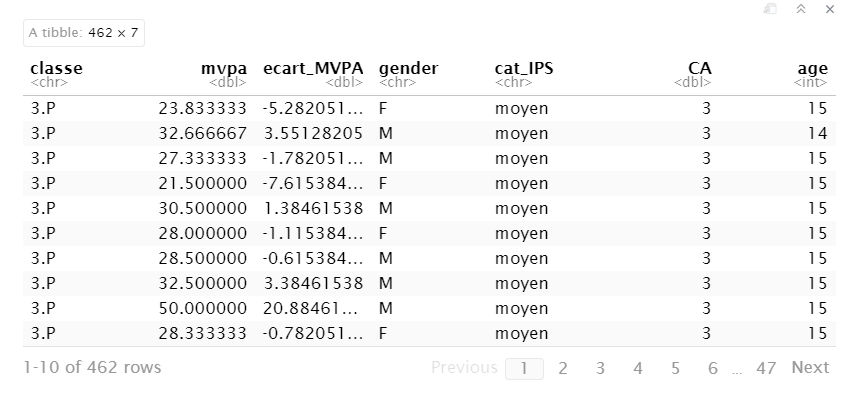
\includegraphics[width=\linewidth]{Extrai_donnée.PNG}
		\caption{Extraits des données}
		\label{fig:image1}
	\end{figure}
	
	
	\textbf{L'objectif de notre étude est d'examiner les écarts de MVPA entre les filles et les garçons en tenant compte de trois variables : la nature de l'activité (CA = champs d'apprentissage), la catégorie socioculturelle de l'établissement (catégorie d'IPS = indice de position sociale) et le milieu géographique.}
	
	\section{Partie Résultats}
	\subsection{Analyse descriptive}
	La première partie de mon stage consiste à faire une analyse descriptive des données après les avoir nettoyées. 
	Les statistiques descriptives sont présentées dans le tableau \ref{tab:descriptive_stats}.
	Au total, nous avons eu 462 participants dans notre étude, dont 220 filles et 242 garçons. Les participants avaient en moyenne 13,65 ans. 47,61\% des participants étaient des filles et 52,39\% étaient des garçons. En termes de champs d'apprentissage, 12,13\% étaient dans le champ 1, 26,15\% dans le champ 2, 10,24\% dans le champ 3 et environ 51,48\% dans le champ 4. En ce qui concerne les catégories d'IPS, 31\% étaient dans la catégorie basse, 22,37\% dans la catégorie moyenne et 46,63\% dans la catégorie haute. Pour les zones géographiques, 64,15\% étaient en zones urbaines et 35,85\% en zones rurales. La moyenne de MVPA pendant 2 heures pour les participants était de 35,14 minutes, avec 31,4 minutes pour les filles et 38,5 minutes pour les garçons. Les détails sur les catégories socio-professionnelles des parents sont présentés dans le tableau \ref{tab:descriptive_stats}, ainsi que le nombre de participants dont les parents occupent l'une des professions listées. Le tableau \ref{tab:descriptive_stats} montre également la proportion de filles et de garçons dans différents champs d'apprentissage, catégories d'IPS et zones géographiques. En général, les proportions de filles et de garçons selon les différentes variables sont similaires, sauf pour certaines modalités de ces variables.
	
	\begin{table}[H]
		\centering
		\begin{tabular}{lrrr}
			\toprule
			\textbf{Variables} & \textbf{Total} & \textbf{Filles} & \textbf{Garçons} \\
			\midrule
			\textbf{Participants} & \textbf{(n = 462)} & \textbf{(n = 220)} & \textbf{(n = 242)} \\
			Participants (\%) & 100\% & 47.61\% & 52.39\%\\
			Âge moyen & 13.65 & 13.66 & 13.65 \\
			\midrule
			\textbf{MVPA}\\
			\textbf{moyenne} & 35.14 & 31.4 & 38.5\\
			\textbf{médiane} & 34.83 & 31 & 37.67\\
			\textbf{écart-type} & 15.79 &  15.23& 15.57 \\
			\textbf{maximum} & 77.16 & 63.5 & 77.17 \\
			\textbf{minimum} &1.333 & 1.33 & 6\\
			\midrule
			\textbf{Catégories socio-professionnelles des parents (nombre)} \\
			Agriculteurs & 10 & 7 & 3 \\
			Artisans, commerçants, chefs d'entreprise & 106 & 59 & 47 \\
			Autres inactifs & 82 & 32 & 50 \\
			Cadres et professions intellectuelles supérieures & 99 & 52 & 47 \\
			Employés & 213 & 90 & 123 \\
			Ouvriers & 66 & 28 & 38 \\
			Professions intermédiaires & 116 & 59 & 57 \\
			Retraités & 7 & 4 & 3 \\
			NA & 43 & 23 & 20 \\
			\midrule
			\textbf{Champs d'apprentissage} \\
			Champ 1 (sports de performance) & 12.13\% & 5.12\% & 7.01\% \\
			Champ 2 (sports de plein air) & 26.15\% & 13.75\% & 12.40\% \\
			Champ 3 (activités artistiques) & 10.24\% & 4.31\% & 5.93\% \\
			Champ 4 (activités d'opposition) & 52.48\% & 24.53\% & 26.95\% \\
			\midrule
			\textbf{Catégories socioculturelles} \\
			Haute & 46.63\% & 16.17\% & 14.83\% \\
			Basse & 22.37\% & 11.86\% & 10.51\% \\
			Moyenne & 31\% & 19.68\% & 26.95\% \\
			\midrule
			\textbf{Zone géographique} \\
			Rurale & 35.85\% & 17.79\% & 18.06\% \\
			Urbaine & 64.15\% & 29.92\% & 34.23\% \\
			\bottomrule
		\end{tabular}
		\caption{Statistiques descriptives des participants}
		\label{tab:descriptive_stats}
	\end{table}
	
	\subsection{Modèles d'ANOVA}
	% Ajouter du contenu ici
	Au total, j'ai fait 3 modèles d'ANOVA trois à deux facteurs pour répondre aux problématiques de mon stage.
	
	\subsubsection{Examen de l'écart de MVPA entre Filles et Garçons selon le CA}
	On souhaite étudier ici l'effet du genre et du champ d'apprentissage sur le MVPA. Pour ce faire, nous utilisons un modèle d'ANOVA à deux facteurs (genre et CA) avec comme variable dépendante l'écart de MVPA à la moyenne de chaque classe. Ce choix de variable dépendante étant imposé par l'étude et est justifié par le fait que certaines classes ont des temps d'activités différents et des enseignants différents, ce qui peut influencer le MVPA mesuré. Ce choix assure donc l'indépendance des observations et l'interprétation revient au même qu'à interpréter directement le MVPA. Dans la suite, 'ecart\_MVPA' fera référence à l'écart de MVPA à la moyenne de chaque classe.
	Pour la contrainte sur le modèle, nous utilisons celle de cellule somme nulle.
	Le modèle s'écrit : 
	\begin{equation}
		Y_{ijk} = \mu + \alpha_i + \beta_j + \gamma_{ij} + \epsilon_{ijk},
	\end{equation}
	$\quad i = 1, \ldots, 2, \quad j = 1, \ldots, 4, \quad k = 1, \ldots, K, \quad \forall i,j,k \quad \epsilon_{ijk} \sim \mathcal{N}(0,\sigma^2)$
	avec un effet moyen général $\mu$, $\alpha_i$ représente l'effet principal du genre, $\beta_j$ représente l'effet principal du CA, un terme d'interaction $\gamma_{ij}$ , les résidus $\epsilon_{ijk}$ avec $k$ l'indice de répétition pour le couple $(i,j)$ et $\sigma^2$ est la variance résiduelle.
	
	\textbf{Plan} :
	On a le tableau de contingence suivant.
	\begin{table}[H]
		\centering
		\begin{tabular}{ccccc}
			\toprule
			& CA 1 & CA 2 & CA 3 & CA 4 \\ 
			\midrule
			F & 20 & 53 & 49 & 98 \\ 
			M & 26 & 51 & 54 & 111 \\ 
			\bottomrule
		\end{tabular}
		\caption{Tableau des CA par genre}
		\label{tab:ca_gender}
	\end{table}
	
	Le nombre d’observations diffère selon le croisement des modalités de CA et gender. Donc nos données sont déséquilibrées, on ne peut donc pas estimer de manière indépendante l’effet d’un facteur ou interactions des autres. Dans ce cas, nous utilisons l'ANOVA de type II car l'ordre des facteurs n'a pas d'importance dans mon étude. Avant de regarder les résultats, nous devons nous assurer que les hypothèses sont validées.
	
	\textbf{Hypothèses du modèle} :
	\begin{itemize}
		\item \textcolor{red}{Indépendance} : L'hypothèse d'indépendance des observations est vérifiée. La liaison qui peut exister due à l'appartenance à une même classe et école est inhibée du fait du choix de l'écart à la moyenne de MVPA de chaque classe au lieu du MVPA.
		\item \textcolor{red}{Homoscédasticité} : 
		Pour valider l'hypothèse d'homoscédasticité, nous visualisons le graphe des résidus en fonction des valeurs prédites.
		\begin{figure}[H]
			\centering
			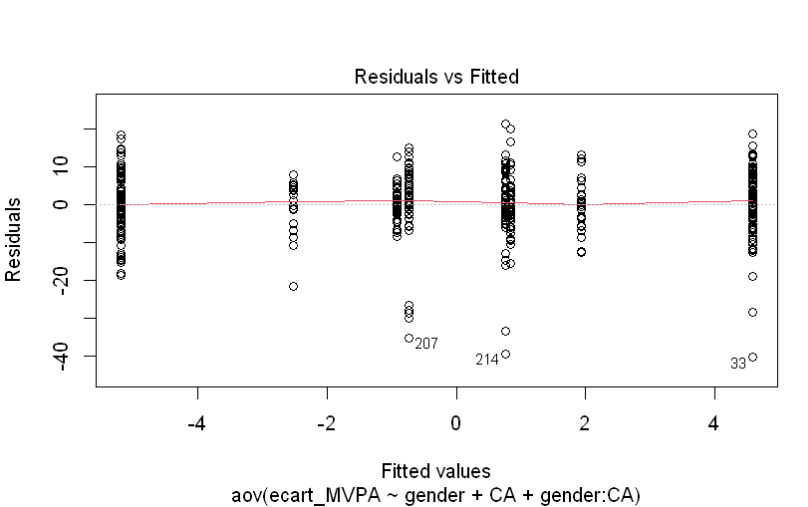
\includegraphics[width=\linewidth]{variance_2.PNG}
			\caption{Graphique de Diagnostic de l'hypothèse d'Homoscédasticité}
			\label{fig:variance2}
		\end{figure}
		Ce graphique nous permet de voir que la variance des résidus est similaire dans tous les groupes.
		\item \textcolor{red}{Normalité des résidus} : 
		Visualisons le graphique du QQ plot.
		\begin{figure}[H]
			\centering
			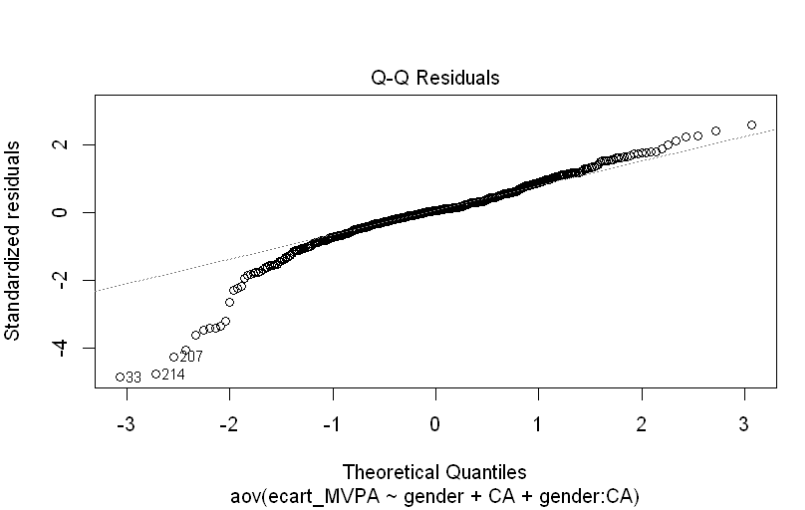
\includegraphics[width=\linewidth]{Normalité_2.PNG}
			\caption{QQ plot}
			\label{fig:qq_plot2}
		\end{figure}
		Le graphique de quantiles contre quantiles permet de vérifier que l'hypothèse de normalité des résidus est raisonnable.
	\end{itemize}
	\textbf{Résultats} : 
	\textit{Test du modèle complet} : 
	On veut tester les hypothèses 
	\begin{itemize}
		\item \textbf{$H_0$} : $\alpha_i = \alpha_{i'}$ et $\beta_j = \beta_{j'}$ et $\gamma_{ij} = \gamma_{i'j'} \quad \forall i' \neq i,\quad j' \neq j$
		\item \textbf{$H_1$} : $\alpha_i \neq \alpha_{i'}$ ou $\beta_j \neq \beta_{j'}$ ou $\gamma_{ij} \neq \gamma_{i'j'} \quad \forall i' \neq i,\quad j' \neq j$
	\end{itemize}
	On a le tableau suivant : 
	\begin{table}[H]
		\centering
		\begin{tabular}{rrrrrrr}
			\toprule
			\textbf{Res.Df} & \textbf{RSS} & \textbf{Df} & \textbf{Sum of Sq} & \textbf{F value} & \textbf{Pr(>F)} \\ 
			\midrule
			461 & 36916 & & & & & \\ 
			454 & 31593 & 7 & 5323.2 & 10.928 & 8.944e-13 *** \\ 
			\bottomrule
		\end{tabular}
		\caption{Tableau des résultats de l'ANOVA}
		\label{tab:anova_results1}
	\end{table}
	La statistique de Fisher $F = \frac{\frac{SCE}{(IJ - 1)}}{\frac{SCR}{(n - IJ)}} = 10.928$ (la variabilité expliquée par le genre et CA est 11 fois supérieure à la variabilité résiduelle), sous $H_0$, $F \sim \mathcal{F}_{7,454}$. Ce qui correspond à une probabilité critique de $8.944 \times 10^{-13}$, donc on rejette $H_0$.
	On peut remarquer que l'ajustement du modèle n'est pas très satisfaisant. En effet, on a $R^2 = 1 - \frac{31593}{36916} = 0.144$.\\
	
	\textit{Test des différents effets} :\\
	On a le tableau suivant : 
	\begin{table}[H]
		\centering
		\begin{tabular}{lrrrr}
			\toprule
			Source & Sum Sq & Df & F value & Pr(>F) \\ 
			\midrule
			gender & 3585.2 & 1 & 51.5200 & 2.911e-12 *** \\ 
			CA & 6.4 & 3 & 0.0307 & 0.9927 \\ 
			gender:CA & 1738.0 & 3 & 8.3252 & 2.122e-05 *** \\ 
			Résidus & 31592.8 & 454 & & \\ 
			\bottomrule
		\end{tabular}
		\caption{Effet des différents facteurs (type II) dans le modèle d'analyse de variance à deux facteurs avec interaction}
		\label{tab:anova_results2}
	\end{table}
	
	\textcolor{blue}{Effet de l'interaction} :\\
	Les hypothèses testées sont  : 
	\begin{itemize}
		\item $H_0$ : Il n'y a pas de différence significative entre le modèle complet et le modèle ne contenant pas l'interaction.
		\item $H_1$ : Il y a une différence significative entre le modèle complet et le modèle ne contenant pas l'interaction.
	\end{itemize}
	La statistique $F_{gender*CA} = 8.3252$, qui sous $H_0$ suis une loi de Fisher à 3 et 454 ddl. La probabilité critique associée au test vaut $2.122\times10^{-5}$. L'effet de l'interaction entre genre et CA est significatif au niveau 0.05. Donc nous n'allons plus accorder trop d'importance au test sur les facteurs principaux, les 2 facteurs sont influents via leur interaction.\\
	
	\textit{Comparaison des ecart\_MVPA} : \\
	Nous avons détecter un effet significatif de l'interaction et ici nous sommes donc intéressé par la différence de ecart\_MVPA entre les filles et garçons selon les différentes CA.
	On veut tester donc les hypothèses : 
	\begin{itemize}
		\item $H_0 : \theta_{i_1j} = \theta_{i_2j}$
		\item $H_1 : \theta_{i_1j} \neq \theta_{i_2j}$
	\end{itemize}
	où $\theta_{i_1j_1}$ et $\theta_{i_2j_2}$ sont les moyennes dans chaque groupe différent et $i_1,i_2\in{\{1, 2\}} $ avec $ i_1 \neq i_2$ ; $j\in{\{1,...,4\}} $.
	Le tableau 8 présente les test post hoc de tukey-kramer, comparaison des moyennes ecart\_MVPA des filles et garçons selon le champs d'apprentissage (CA)
	\begin{table}[H]
		\centering
		\begin{tabular}{|p{5cm}|c|c|c|c|}
			\hline
			& CA1 & CA2 & CA3 & CA4 \\ 
			\hline
			Écart moyen entre fille et garçon des écarts à la moyenne de MVPA de chaque classe & -4.4548 & -1.4898 & -1.7470 & -9.7647 \\ 
			\hline
			Intervalle de confiance & -12.010 à 3.100 & -6.4730 à 3.493 & -6.759 à 3.265 & -13.286 à -6.244 \\ 
			\hline
			P-valeur & 0.6235 & 0.9850 & 0.96 & 0.000 \\ 
			\hline
		\end{tabular}
		\caption{ Test de comparaison des moyennes de ecrat\_MVPA des filles et garçon dans les CA différents}
		\label{tab:ecarts_mvpa}
	\end{table}
	
	Le MVPA (ou ecart\_MVPA car ils ont même interprétation) des garçons est significativement supérieur à celui des filles dans le champ 4 (p\_valeur < .05, on rejette $H_0$) par contre dans les autres champs cette différence n'est pas significative avec des p\_valeur largement supérieur à 5\% (on conserve $H_0$).\\
	Le graphe ci-dessous résume cette situation	:
	\begin{figure}[H]
		\centering
		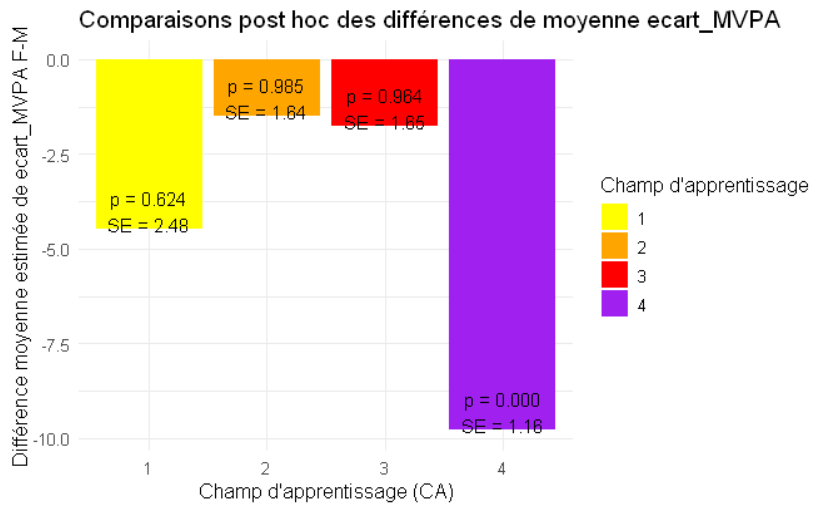
\includegraphics[width=\linewidth]{Diagramme_1.PNG}
		\caption{Diagramme en barre représentatif des test de comparaison des moyennes de ecrat\_MVPA des filles et garçon dans les CA différents avec les p-valeur et écart\_type}
		\label{fig:Test post hoc}
	\end{figure}
	\textbf{On voit clairement sur ce graphe que dans le champ 4 les garçons s'impliquent plus que les filles ce qui n'est clairement pas le cas dans les autres champs d'apprentissage.}
	
	\textit{Taille d'effet} : \\
	Dans le champ 4 il y a une différence significative de moyenne ecart\_MVPA entre les filles et garçons ce qui est traduit par un effet significatif de l'interaction entre le genre et CA. La question qu'on se pose est de savoir quelle est la force de cet effet.\\
	On a les résultats suivants : \\
	\begin{table}[H]
		\centering
		\begin{tabular}{ccc}
			\toprule
			Parameter & $\omega^2$ & 95\% CI \\
			\midrule
			gender & 0.10 & [0.06, 1.00] \\
			CA & 0.00 & [0.00, 1.00] \\
			gender:CA & 0.05 & [0.02, 1.00] \\
			\bottomrule
		\end{tabular}
		\caption{Tableau des tailles d'effet ($\omega^2$) et intervalle de confiance à 95\% (unilatéral)}
		\label{table:2}
	\end{table}
	\textbf{La taille d'effet pour l'interaction entre genre et CA est 0.05 ce qui signifie que 5\% de la variance totale de la variable dépendante (ecart\_mvpa) peut être attribuée à l'effet de l'interaction. Dans le métier cette taille d'effet est modérément importante ce qui nous permet de tenir compte de ce résultat dans la pratique (écart de mvpa entre les filles et garçons observé dans le champ 4 est à prendre en compte dans la pratique car jugé important).}
	
	\subsubsection{Examen de l'écart de MVPA entre Filles et Garçons}
	L'objectif ici est de voir si l'étude fait produit un résultat similaire à ceux des travaux antérieurs.
	\subsubsection{Examen de l'écart de MVPA entre Filles et Garçons selon la catégorie IPS}
	L'objectif ici est d'examiner l'effet du genre et de la catégorie IPS sur le MVPA. Nous utilisons donc un modèle d'ANOVA à deux facteurs (genre et IPS catégorie) avec comme variable dépendante ecart\_MVPA. Pour la contrainte sur le modèle, nous utilisons celle de somme des coefficients nulle.
	Le modèle s'écrit :
	\begin{equation}
		Y_{ijk} = \mu + \alpha_i + \beta_j + \gamma_{ij} + \epsilon_{ijk},
	\end{equation}
	$\quad i = 1, \ldots, 2, \quad j = 1, \ldots, 3, \quad k = 1, \ldots, K, \quad \forall i,j,k \quad \epsilon_{ijk} \sim \mathcal{N}(0,\sigma^2)$
	avec un effet moyen général $\mu$, $\alpha_i$ représente l'effet principal du genre, $\beta_j$ représente l'effet principal de l'IPS catégorie, un terme d'interaction $\gamma_{ij}$ , les résidus $\epsilon_{ijk}$ avec $k$ l'indice de répétition pour le couple $(i,j)$ et $\sigma^2$ est la variance résiduelle. 
	
	\textbf{Plan}: On a le tableau de contingence suivant
	\begin{table}[H]
		\centering
		\begin{tabular}{cccc}
			\toprule
			& Élevée & Faible & Moyenne \\
			\midrule
			F & 93 & 48 & 79 \\
			M & 89 & 44 & 109 \\
			\bottomrule
		\end{tabular}
		\caption{Tableau de contingence entre le genre et l'IPS catégorie}
		\label{table:1}
	\end{table}
	On voit clairement que nos données sont déséquilibrées. Nous utilisons donc une ANOVA de Type II. En effet, l'ordre d'insertion des facteurs dans le modèle n'est pas important dans le cadre de mon étude.
	Avant de regarder les résultats, nous devons nous assurer que les hypothèses du modèle sont validées.\\
	\textbf{Hypothèses du modèle} :
	\begin{itemize}
		\item \textcolor{red}{Indépendance} : L'hypothèse d'indépendance des observations est vérifiée.
		\item \textcolor{red}{Homoscédasticité} : 
		Pour valider l'hypothèse d'homoscédasticité, nous visualisons le graphe des résidus en fonction des valeurs prédites.
		\begin{figure}[H]
			\centering
			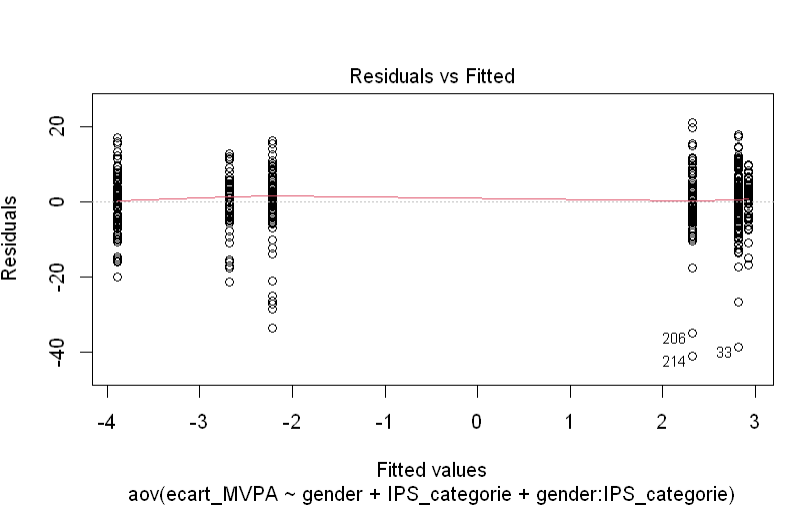
\includegraphics[width=\linewidth]{variance_3.PNG}
			\caption{Graphique de Diagnostic de l'hypothèse d'Homoscédasticité}
			\label{fig:variance2}
		\end{figure}
		Ce graphique nous permet de voir que la variance des résidus est similaire dans tous les groupes.
		\item \textcolor{red}{Normalité des résidus} : 
		Visualisons le graphique du QQ plot.
		\begin{figure}[H]
			\centering
			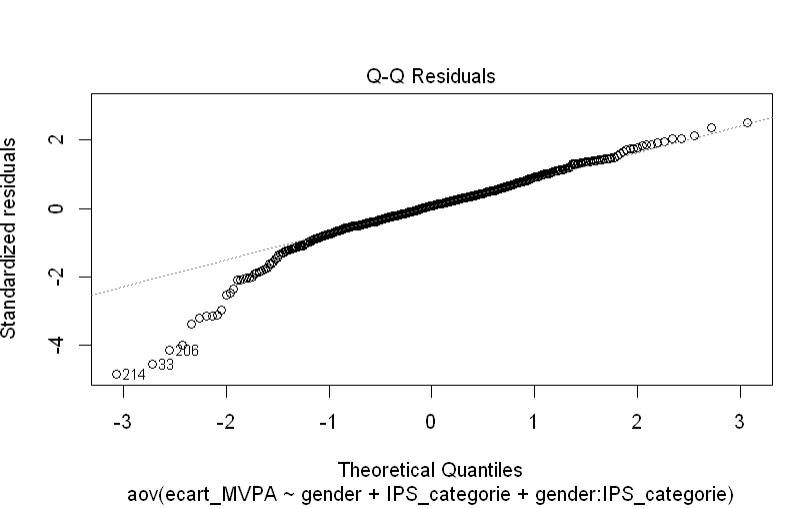
\includegraphics[width=\linewidth]{Normalité_3.PNG}
			\caption{QQ plot}
			\label{fig:qq_plot2}
		\end{figure}
		Le graphique de quantiles contre quantiles permet de vérifier que l'hypothèse de normalité des résidus est raisonnable.
	\end{itemize}
	
	\textbf{Résultats} : \\
	\textit{Test du modèle complet} : \\
	On veut tester les hypothèses 
	\begin{itemize}
		\item \textbf{$H_0$} : $\alpha_i = 0$ et $\beta_j = 0$ et $\gamma_{ij} = 0 \quad \forall i,j$
		\item \textbf{$H_1$} :$\alpha_i \neq 0$ ou $\beta_j \neq 0$ ou $\gamma_{ij} \neq 0 \quad \forall i,j$
	\end{itemize}
	On a le tableau suivant : 
	\begin{table}[H]
		\centering
		\begin{tabular}{rrrrrrr}
			\toprule
			\textbf{Res.Df} & \textbf{RSS}  & \textbf{Df} & \textbf{Sum of Sq} & \textbf{F} & \textbf{Pr(>F)} \\ 
			\midrule
			461 & 36916 &    &           &        &           \\ 
			456 & 33199 &  5 & 3717.1    & 10.211 & 2.74e-09 *** \\ 
			\bottomrule
		\end{tabular}
		\caption{Tableau des résultats de l'analyse de variance}
		\label{table:3}
	\end{table}
	La statistique de Fisher $F = \frac{\frac{SCE}{(IJ - 1)}}{\frac{SCR}{(n - IJ)}} = 10.211$ (la variabilité expliquée par le genre et L'IPS catégorie est 10 fois supérieure à la variabilité résiduelle), sous $H_0$, $F \sim \mathcal{F}_{5,456}$. Ce qui correspond à une probabilité critique de $2.74 \times 10^{-09}$, donc on rejette $H_0$.
	On peut remarquer que l'ajustement du modèle n'est pas très satisfaisant. En effet, on a $R^2 = 1 - \frac{33199}{36916} = 0.1006$.\\
	
	\textit{Test des différents effets} : \\
	On a le tableau suivant : 
	\begin{table}[H]
		\centering
		\begin{tabular}{lrrrr}
			\toprule
			Source & Sum Sq & Df & F value & Pr(>F) \\ 
			\midrule
			gender                & 3610   & 1  & 49.5860 & 7.028e-12 *** \\ 
			IPS\_categorie        & 31     & 2  & 0.2152  & 0.8064    \\ 
			gender:IPS\_categorie & 107    & 2  & 0.7349  & 0.4801    \\ 
			Residuals             & 33199  & 456 &         &           \\ 
			\bottomrule
		\end{tabular}
		\caption{Tableau des résultats de l'analyse de variance pour l'effet du genre et de la catégorie IPS}
		\label{tab:anova_results3}
	\end{table}
	\textcolor{blue}{Effet de l'interaction}\\
	Ici nous testons les hypothèses 
	\begin{itemize}
		\item \textbf{$H_0$} : $Y_{ijk} = \mu + \alpha_i + \beta_j + \epsilon_{ijk} \quad \forall i,j,k$ 
		\item \textbf{$H_1$} : $Y_{ijk} = \mu + \alpha_i + \beta_j + \gamma_{ij} + \epsilon_{ijk} \quad \forall i,j,k$
	\end{itemize}
	La statistique de test $F_{gender*IPS\_categorie} = 0.7349$, qui sous $H_0$ suit une loi de Fisher à 2 et 456 ddl. La p-valeur associé au test vaut 0.4801 donc l'hypothèse de non interaction $H_0$ est conservée.\\
	
	\textcolor{blue}{Effet de l'IPS\_catégorie}\\
	Nous souhaitons savoir si l'IPS\_categorie possède un effet sur ecart\_MVPA. Nous testons alors les hypothèses 
	\begin{itemize}
		\item \textbf{$H_0$} : $Y_{ijk} = \mu + \alpha_i + \epsilon_{ijk} \quad \forall i,j,k$ 
		\item \textbf{$H_1$} : $Y_{ijk} = \mu + \alpha_i + \beta_j + \epsilon_{ijk} \quad \forall i,j,k$
	\end{itemize}
	La statistique de test $F_{IPS\_categorie}=0.2152$ qui sous $H_0$ suit une loi de Fisher à 2 et 456 ddl. La p-valeur observé vaut 0.8064 donc nous conservons $H_0$, il n'existe pas d'effet de l'IPS\_categorie sur ecart\_MVPA.\\
	
	\textbf{Donc l'écart de MVPA entre fille et garçons ne dépendent pas de la catégorie socio-professionnelle}.
	
	\subsubsection{Examen de l'écart de MVPA entre Filles et Garçons selon le milieu géographique}
	Afin de savoir si les variables genre et milieu géographique ont un effet sur le MVPA, nous allons utiliser une ANOVA à deux facteurs (genre et géographie) avec comme variable dépendante ecrat\_MVPA. Pour la contrainte sur le modèle, nous utilisons celle de somme des coefficients nulle. \\
	Le modèle s'écrit : 
	\begin{equation}
		Y_{ijk} = \mu + \alpha_i + \beta_j + \gamma_{ij} + \epsilon_{ijk},
	\end{equation}
	$\quad i = 1, \ldots, 2, \quad j = 1, \ldots, 4, \quad k = 1, \ldots, K, \quad \forall i,j,k \quad \epsilon_{ijk} \sim \mathcal{N}(0,\sigma^2)$
	avec un effet moyen général $\mu$, $\alpha_i$ représente l'effet principal du genre, $\beta_j$ représente l'effet principal du milieu géographique, un terme d'interaction $\gamma_{ij}$ , les résidus $\epsilon_{ijk}$ avec $k$ l'indice de répétition pour le couple $(i,j)$ et $\sigma^2$ est la variance résiduelle.\\
	
	\textbf{Plan} : \\
	Nous obtenons le tableau de contingence suivant
	\begin{table}[H]
		\centering
		\begin{tabular}{ccc}
			\toprule
			& Rural & Urbain \\
			\midrule
			F & 101 & 119 \\
			M & 102 & 140 \\
			\bottomrule
		\end{tabular}
		\caption{Tableau de contingence}
		\label{tab:tab_contingence}
	\end{table}
	Les données sont déséquilibrées, nous utiliserons donc une ANOVA de type II (l'ordre d'insertions des facteurs dans le modèle n'a pas d'importance). Avant de regarder les résultats, nous devons nous assurer que les hypothèses du modèle sont validées.\\
	\textbf{Hypothèses du modèle}:\\
	\textit{Indépendance}: L'hypothèse d'indépendance des observations est vérifiée.\\
	\textit{Homoscédasticité}: Visualisons le graphe des résidus en fonction des valeurs prédites.
	\begin{figure}[H]
		\centering
		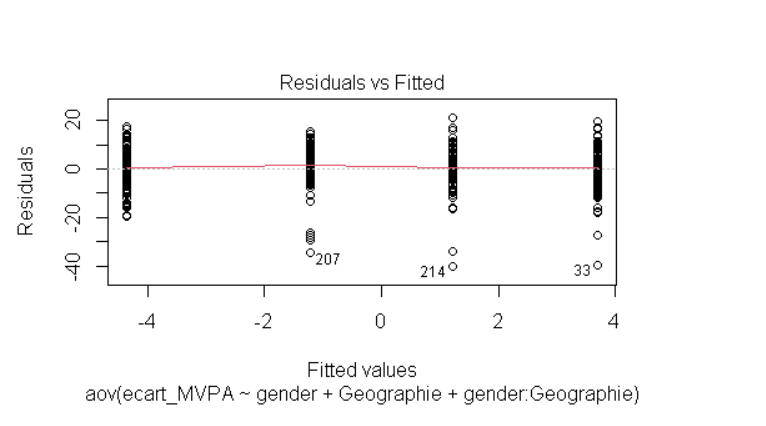
\includegraphics[width=\linewidth]{variance_4.PNG}
		\caption{Graphique de Diagnostic de l'hypothèse d'Homoscédasticité}
		\label{fig:variance2}
	\end{figure}
	Ce graphique nous permet de voir que la variance des résidus est similaire dans tous les groupes.\\
	\textit{Normalité des résidus}: Visualisons le graphique du QQ-plot.
	\begin{figure}[H]
		\centering
		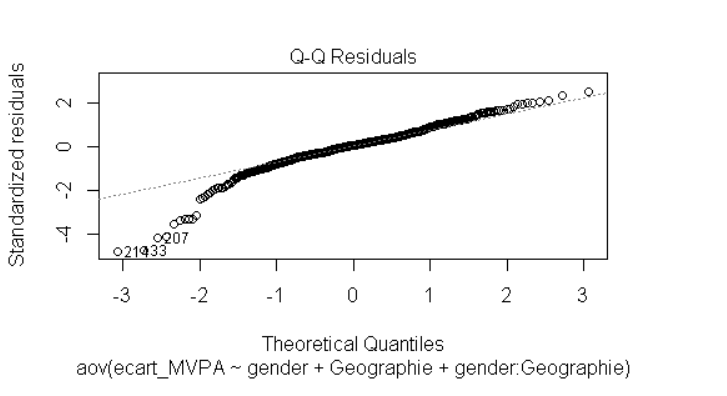
\includegraphics[width=\linewidth]{Normalité_4.PNG}
		\caption{QQ plot}
		\label{fig:qq_plot2}
	\end{figure}
	Le graphique de quantile contre quantile permet de vérifier que l'hypothèse de normalité des résidus est raisonnable.\\
	
	\textbf{Résultats} : \\
	\textit{Test du modèle complet} : \\
	On souhaite tester
	\begin{itemize}
		\item $H_0 : \alpha_i = 0$ et $\beta_j = 0$ et $\gamma_{ij} = 0 \quad \forall i,j$ 
		\item $H_1 : \alpha_i = 0$ ou $\beta_j = 0$ ou $\gamma_{ij} = 0 \quad \forall i,j$ 
	\end{itemize}
	Voici les résultats :
	\begin{table}[H]
		\centering
		\begin{tabular}{rrrrrl}
			\toprule
			\textbf{Res.Df} & \textbf{RSS} & \textbf{Df} & \textbf{Sum of Sq} & \textbf{F} & \textbf{Pr(>F)} \\
			\midrule
			461 & 36916 &    &         &         &        \\
			458 & 32439 &  3 & 4477.3  & 21.072  & 8.375e-13 *** \\
			\bottomrule
		\end{tabular}
		\caption{Tableau des résultats de l'analyse de variance}
		\label{tab:anova_results}
	\end{table}
	La statistique de test $F = \frac{\frac{SCE}{(IJ - 1)}}{\frac{SCR}{(n - IJ)}} = 21.072$ (la variabilité expliquée par le genre et le milieu géographique est 21 fois supérieure à la variabilité résiduelle), sous $H_0$, $F \sim \mathcal{F}_{3,458}$. Ce qui correspond à une probabilité critique de $8.375 \times 10^{-13}$, donc on rejette $H_0$.
	On peut remarquer que l'ajustement du modèle n'est pas très satisfaisant. En effet, on a $R^2 = 1 - \frac{32439}{36916} = 0.1212$.\\
	
	\textit{Test des différents effets} : \\
	On obtient le tableau ci-dessous : 
	\begin{table}[H]
		\centering
		\begin{tabular}{lrrrr}
			\toprule
			& Sum Sq & Df & F value & Pr(>F)     \\
			\midrule
			gender            & 3584   & 1  & 50.6006 & 4.386e-12  \\
			Geographie        & 5      & 1  & 0.0725  & 0.7879208  \\
			gender:Geographie & 893    & 1  & 12.6145 & 0.0004224  \\
			Residuals         & 32439  & 458 &         &            \\
			\bottomrule
		\end{tabular}
		\caption{Analysis of Variance Table}
	\end{table}
	\textcolor{blue}{Effet de l'interaction} \\
	On souhaite tester : 
	\begin{itemize}
		\item \textbf{$H_0$} : $Y_{ijk} = \mu + \alpha_i + \beta_j + \epsilon_{ijk} \quad \forall i,j,k$ 
		\item \textbf{$H_1$} : $Y_{ijk} = \mu + \alpha_i + \beta_j + \gamma_{ij} + \epsilon_{ijk} \quad \forall i,j,k$
	\end{itemize}
	La statistique de test $F_{gender*geographie} = 12.6145$, qui sous $H_0$ suit une loi de Fisher à 1 et 458 ddl. La p-valeur associé au test vaut 0.0004224 donc l'effet de l'interaction entre genre et milieu géographique est significatif au niveau de 5\%. Les deux facteurs sont influents via leur interaction, il n'est donc pas nécessaire de tester leur influence respective.\\
	
	\textit{Comparaison des ecarts\_MVPA} :\\
	Un effet significatif de l'interaction est détecter et ici nous sommes intéressé par la différence de ecart\_MVPA entre les filles et garçons selon les différents milieu géographique. On veut tester les hypothèses : 
	\begin{itemize}
		\item $H_0 : \theta_{i_1j} = \theta_{i_2j}$
		\item $H_1 : \theta_{i_1j} \neq \theta_{i_2j}$
	\end{itemize}
	où $\theta_{i_1j_1}$ et $\theta_{i_2j_2}$ sont les moyennes dans chaque groupe différent et $i_1,i_2\in{\{1, 2\}} $ avec $ i_1 \neq i_2$ ; $j\in{\{1,2\}}$.
	Le tableau suivant présente la comparaison des ecart\_MVPA des filles et garçons selon le champs d'apprentissage
	\begin{table}[H]
		\centering
		\begin{tabular}{|p{5cm}|c|c|}
			\hline
			& Rural & Urbain \\ 
			\hline
			Écart entre filles et garçons des écarts à la moyenne de MVPA de chaque classe & -2.44 & -8.06 \\ 
			\hline
			Intervalle de confiance & -5.49 à 0.602 & -10.761 à -5.350 \\ 
			\hline
			P-valeur & 0.1650 & 0.000 \\ 
			\hline
		\end{tabular}
		\caption{Comparaison des écarts à la moyenne de MVPA par genre et par localisation}
		\label{tab:ecarts_mvpa_genre_localisation}
	\end{table}
	Le MVPA (ou ecart\_MVPA) est significativement supérieur à celui des filles dans le milieu urbain (p-valeur <.05, on rejette $H_0$) par contre dans le milieu rural cette différence n'est pas significative (p-valeur > .05, on conserve $H_0$).\\
	Le graphe ci-dessous résume cette situation :
	\begin{figure}[H]
		\centering
		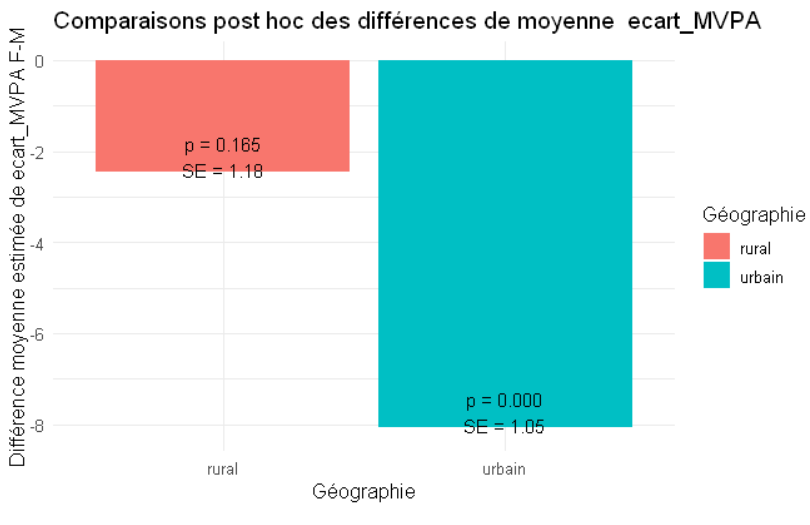
\includegraphics[width=\linewidth]{Diagramme_2.PNG}
		\caption{Diagramme en barre représentatif des test de comparaison des moyennes de ecrat\_MVPA des filles et garçon dans les CA différents avec les p-valeur et écart\_type}
		\label{fig:Test post hoc}
	\end{figure}
	\textbf{On voit clairement sur ce graphe que dans le milieu urbain les garçons s'impliquent plus que les filles ce qui n'est pas clairement le cas en milieu rural.}
	
	\textit{Taille d'effet} :
	En milieu urbain il y a une différence significative de moyenne eacrt\_MVPA entre fille et garçon ce qui est traduit par un effet significatif de l'interaction entre le genre et le milieu géographique. Ici la question qu'on se pose est de savoir quelle est la force de ce effet.\\
	On a le tableau suivant : 
	\begin{table}[H]
		\centering
		\begin{tabular}{|l|c|c|}
			\hline
			\textbf{Parameter} & \textbf{$\omega^2$} & \textbf{95\% CI} \\
			\hline
			gender             & 0.10                      & [0.06, 1.00]      \\
			Geographie         & 0.00                      & [0.00, 1.00]      \\
			gender:Geographie  & 0.02                      & [0.01, 1.00]      \\
			\hline
		\end{tabular}
		\caption{Taille d'effet $\omega^2$ et intervalle de confiance à 95\% (unilatéral)}
		\label{table:omega2}
	\end{table}
	\textbf{La taille d'effet pour l'interaction entre genre et milieu géographique est 0.02 ce qui signifie que 5\% de la variance totale de la variable dépendante (ecart\_MVPA) peu être attribuée à l'effet de l'interaction. Dans le métier cette taille d'effet est faible. La différence de ecart\_MVPA entre fille et garçon observé en milieu urbain existe belle et bien mais cette doifférence n'est pas assez important pour en tenir compte dans la pratique.}
	\section{Discusion sur les limites des résultats}
	Il est à noté que le calcul et l'interprétation des résultats de la taille d'effet est dans le cas de plan non équilibré un peu plus complexe du au fait qu'une partie de la variance est manquante. En effet comme la variabilité totale ne peut pas être décomposé en la variabilité des différents effet donc certaine variabilité qui ne peuvents pas être attribué à un effet spécifique disparais dans le cas de l'ANOVA de type II ou III. Donc même si la taille d'effet n'ai pas assez précis dans le cas de plan non équilibré, il nous donne quand même un vision globale sur la force de l'effet du facteur (plan pas trop déséquilibré).
	\section{Conclusion}
	% Ajouter du contenu ici
	
\end{document}
